% Created 2022-12-07 Wed 13:23
% Intended LaTeX compiler: pdflatex
\documentclass[a4paper,11pt]{article}
\usepackage[utf8]{inputenc}
\usepackage[T1]{fontenc}
\usepackage{graphicx}
\usepackage{longtable}
\usepackage{wrapfig}
\usepackage{rotating}
\usepackage[normalem]{ulem}
\usepackage{amsmath}
\usepackage{amssymb}
\usepackage{capt-of}
\usepackage{hyperref}
\usepackage[margin=1in]{geometry}
\usepackage{titlesec}
\usepackage{caption}
\usepackage{subcaption}
\usepackage{lipsum}
\author{Varghese Reji}
\date{}
\title{Classical and Quantum Optics\\\medskip
\large Assignment-2 Answers}
\hypersetup{
 pdfauthor={Varghese Reji},
 pdftitle={Classical and Quantum Optics},
 pdfkeywords={},
 pdfsubject={},
 pdfcreator={Emacs 28.2 (Org mode 9.5.5)}, 
 pdflang={English}}
\begin{document}

\maketitle

\section*{Problem 1}
\label{sec:org016a999}

The python code to solve this question is given \href{https://github.com/varghesereji/Coursework\_assignments/blob/main/APP/Ass2/Problem\_1.py}{here}.


To create the upper confidence limit, we use the formula,

\begin{equation}
\label{eq:org0023ef4}
P(x<x_1|\mu)=1-\alpha
\end{equation}

and for central interval, we use

\begin{equation}
\label{eq:org461749e}
P(x<x_1|mu)=P(x>x_2)=\frac{(1-\alpha)}{2}
\end{equation}

We will take the central interval 68\% and upper limit 90\%.

\begin{description}
\item[{(a)}] Poisson Discrete random variable.
\end{description}
\begin{equation}
\label{eq:orge557627}
P(x|\mu) = \frac{\mu^x}{x!}e^{-\mu}
\end{equation}

The plots are shown below.

\begin{center}
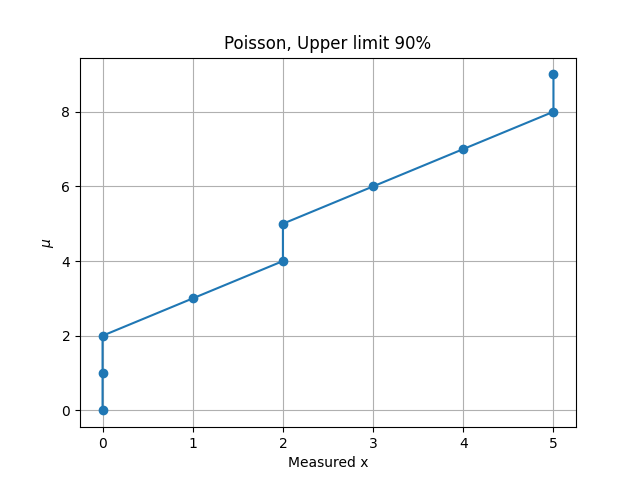
\includegraphics[width=.9\linewidth]{poisson_upper.png}
\end{center}

\begin{center}
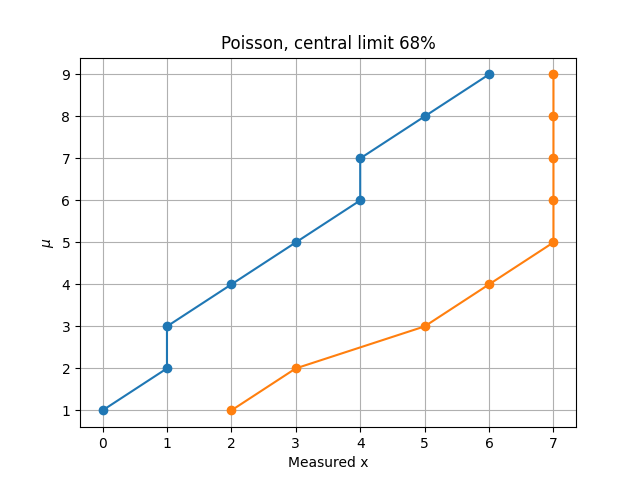
\includegraphics[width=.9\linewidth]{poisson_central.png}
\end{center}

\begin{description}
\item[{(b)}] Uniform distribution. Here, \(k=2\mu\).

Here, I took \(k=100\). Plots are shown here.
\begin{center}
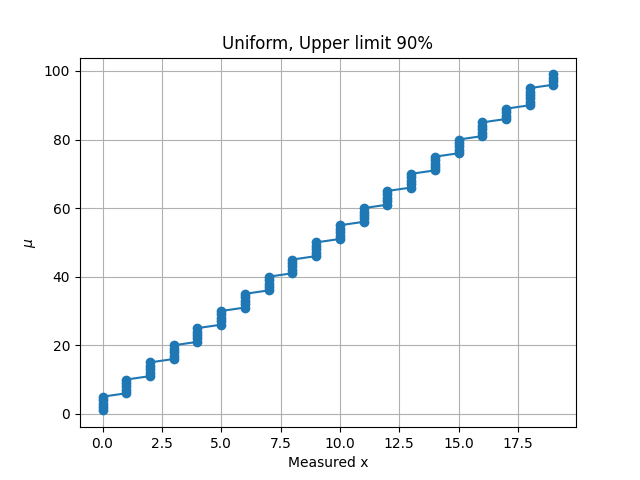
\includegraphics[width=.9\linewidth]{uniform_upper.png}
\end{center}

\begin{center}
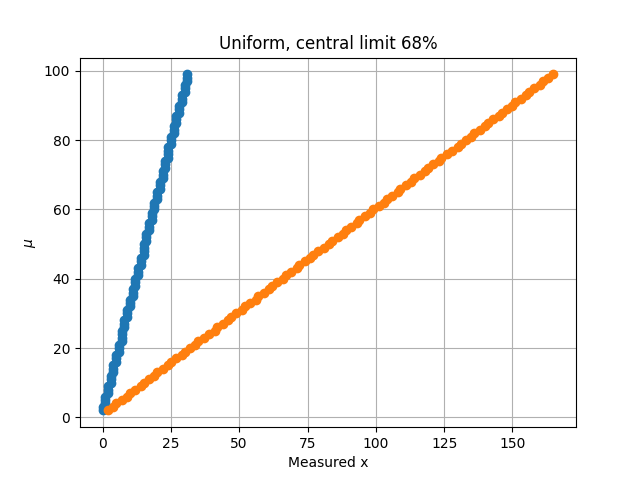
\includegraphics[width=.9\linewidth]{uniform_central.png}
\end{center}

\item[{(c)}] Gaussian function with \(\sigma=1\).
\end{description}


\begin{equation}
\label{eq:org777366e}
P(x|\mu) = \frac{1}{\sqrt{2\pi}} \exp\left(\frac{(x-\mu)^2}{2}\right)
  \end{equation}


\begin{center}
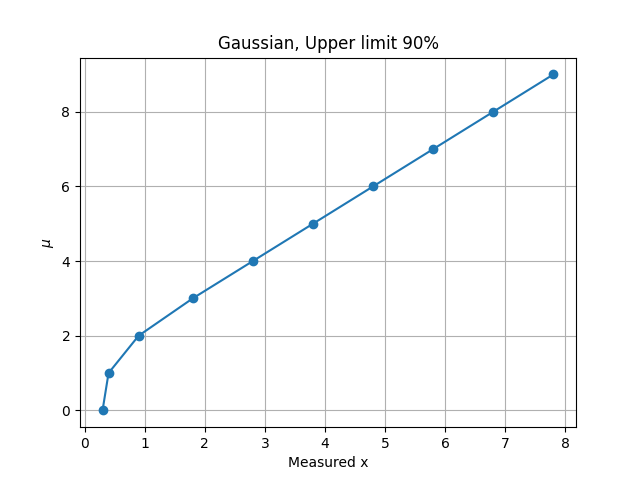
\includegraphics[width=.9\linewidth]{gaussian_upper.png}
\end{center}

\begin{center}
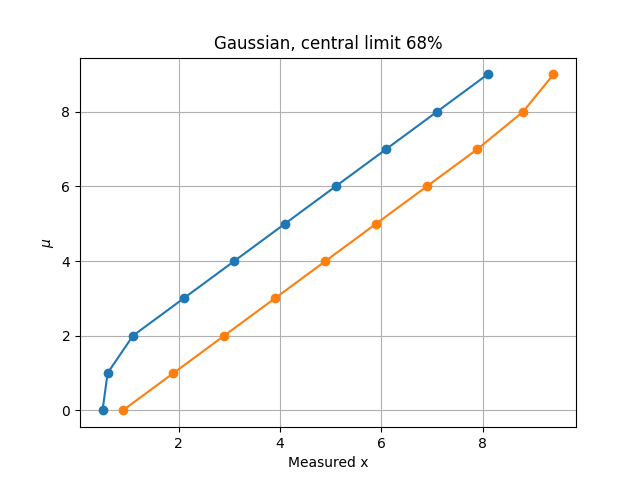
\includegraphics[width=.9\linewidth]{gaussian_central.png}
\end{center}
\end{document}